Now that we have understood classical mechanics and quantum mechanics as probability theories and displayed their differences, we will now concern ourselves with the development of algebraic methods that will allow us to describe both classical and quantum mechanics in the same framework and to discuss equilibrium further. We will define the notions of $C^*$-algebras, von Neumann algebras, dynamical systems, and develop the GNS construction. Through examples we will see the physical importance of these concepts. 
 
\section{C*-algebras}

We will start by getting acquainted with the notion of a $C^*$-algebra. This is the mathematical structure we will endow our physical observables with. Even though the general need for this structure can be inspired by the abstract analysis of experimental apparatuses\cite{Strocchi2008a} we will instead give the abstract definition and then justify it through examples. 

\begin{definition}
An (associative) algebra $\mathcal{A}$ is a set equipped with three operations:
\begin{align}
\begin{split}
 \mathcal{A} \times \mathcal{A} & \rightarrow  \mathcal{A} \\
 (A,B) & \mapsto  A+B \quad\text{addition;}  \\
 \mathbb{C} \times \mathcal{A} & \rightarrow \mathcal{A} \\
 (\lambda,A) & \mapsto \lambda A \quad\text{scalar multiplication;} \\
 \mathcal{A} \times \mathcal{A} & \rightarrow \mathcal{A} \\
 (A, B) & \mapsto AB \quad\text{multiplication;}
\end{split}
\end{align}
such that with addition and scalar multiplication it forms a complex vector space, with addition and multiplication it forms a ring, and there is a compatibility condition between scalar multiplication and multiplication, which is that for all $A,B\in\mathcal{A}$ and $\lambda\in\mathbb{C}$ we have $(\lambda A)B=A(\lambda B) = \lambda (AB)$. If the ring is commutative the algebra is said to be commutative and if the ring is unital the algebra is said to be unital. A norm on an algebra $\mathcal{A}$ is a norm on the vector space structure $\|\cdot\|:\mathcal{A} \rightarrow \mathbb{R}^{+}_0 $ such that for all $A,B\in\mathcal{A}$ we have $\|AB\|\leq\|A\|\|B\|$. An algebra endowed with a norm is called a normed algebra. If the normed vector space structure of an algebra is Banach, the algebra is called Banach. An involution on an algebra $\mathcal{A}$ is a map $^*:\mathcal{A}  \rightarrow \mathcal{A} \quad A \mapsto A^*$ such that for all $A,B\in\mathcal{A}$ and $\lambda\in\mathbb{C}$:
\begin{align}
\begin{split}
(\lambda A + B)^*&=\bar{\lambda}A^* + B^*; \\
(AB)^*&=B^*A^*;\\
(A^*)^*&=A.
\end{split}
\end{align}
An algebra equipped with an involution is said to be a *-algebra. A $C^*$-algebra is a Banach *-algebra where for all $x\in\mathcal{A}$ 
\begin{equation}
\|A^*A\|=\|A\|^2.
\end{equation}
\end{definition}

\begin{example}
The set of continuous functions vanishing at infinity on a locally compact Hausdorff space $X$, that is the set $C_0(X)$ of continuous $f:X\rightarrow \mathbb{C}$ such that for every $\epsilon\in\mathbb{R}^+$ there exists a compact set $K$ such that $f(K^c)\subseteq B(0,\epsilon) \subseteq \mathbb{C}$ forms a $C^*$-algebra with the supremum norm
\begin{equation}
\|f\| = \sup\{|f(x)||x\in X\}.
\end{equation}
This algebra differs from the structure described in \ref{sec:classical_probability} in that the behavior of the functions at infinity is restricted. Nevertheless $C_0(X)$ is unital if and only if $X$ is compact. In that case $C_0(X)=C(X)$ and the observables coincide with the self-adjoint elements of the $C^*$-algebra. One can associate both the need for restricting behavior at infinity or making the space compact by noting that any real feasible experiment performed on a system should be localized. This has to do with the experimental motivation of $C^*$-algebras given in \cite{Strocchi2008a}.
We now note that every commutative $C^*$-algebra can be realized as the space $C_0(X)$ for $X$ a locally compact Hausdorff space\cite{Bratteli1997}. 
\end{example}

\begin{example}
The set of bounded operators in a Hilbert space $\mathcal{H}$ forms a $C^*$-algebra with the operator norm
\begin{equation}
\|A\|=\sup\left\{\left.\frac{\|Ax\|}{\|x\|}\right|x\in\mathcal{H}\setminus \{0\} \right\}.
\end{equation}
Moreover, every closed self-adjoint subspace of the bounder operators $\mathcal{B}(\mathcal{H})$ of a Hilbert space $\mathcal{H}$ is a $C^*$-algebra. Conversely, the Gelfand-Naimark theorem shows that every $C^*$-algebra is realizable as a closed self-adjoint subspace of $\mathcal{B}(\mathcal{H})$ for some Hilbert space $\mathcal{H}$\cite{Bratteli1997}. Once again, this algebra differs from the structure given in section \ref{sec:QM} because we only consider bounded operators. Once again at a fundamental level this does not matter since we know through the spectral theorem or the logical structure presented in section \ref{sec:Q_logic} that we can describe all observables (bounded or unbounded) through their spectral decomposition into projections. In particular, we should be able to take the $C^*$-algebra generated by the projections associated to the observable we want to analyze. For example, instead of considering the position operator $q$ on $L^2(\mathcal{H})$ given by $q\psi(x)=x\psi(x)$ for all $\psi\in\mathcal{H}$, we can consider the $C^*$-algebra generated by the characteristic functions of Borel sets $E\subseteq\mathbb{R}$ whose action on the Hilbert space is $\chi_E\psi(x) = \chi_E(x)\psi(x)$. Moreover, this problem, as in the classical case, is related to the fact that no experimental apparatus has an infinite display of outcomes. One indeed cannot measure infinitely large positions or momenta.

Another solution for the case of Schrödinger's mechanics is to consider the Weyl operators $U(a)$ and $U(b)$ for $a,b\in\mathbb{R}$ given by
\begin{align}
\begin{split}
U(a)\psi(x) &= \psi(x-\hbar a) \\
V(b)\psi(x) &= e^{-ibx}\psi(x).
\end{split} 
\end{align}
By Stone's theorem if $q$ is the position operator and $p$ is the momentum operator satisfying the canonical commutation relations $[x,p]=i\hbar$ we have $U(a)=e^{-iap}$ and $V(b)=e^{-ibq}$\cite{Strocchi2008a}. 
\end{example}

As mentioned before the above definition gives structure to the observables of a system. To get a complete kinematical description we need to also give structure to the notion of state. We can inspire the definition of a state by the fact that both in classical and quantum descriptions the statistically appropriate notion of state seemed to act on the observable either through equation \ref{eq:classical_states} or \ref{eq:quantum_states}.

\begin{definition}
A state on a $C^*$-algebra $\mathcal{A}$ is a positive normalized linear functional $\omega:\mathcal{A}\rightarrow \mathbb{C}$, i.e. it is a linear map such that $\|\omega\| = 1$ (normalized) and for all $A\in\mathcal{A}$ we have $\omega(A^*A)\geq 0$ (positive). If $\omega(A^*A)>0$ for all $A\in\mathcal{A}\setminus\{0\}$, the state is said to be faithful.
\end{definition}  

Note that for a unital $C^*$-algebra a positive linear functional $\omega$ is normalized if and only if $\omega(1)=1$\cite{Bratteli1997}.

Some useful facts about states are included in the next theorem\cite{Bratteli1997}.

\begin{theorem}
Let $\omega$ be a state on a $C^*$-algebra $\mathcal{A}$. Then for all $A,B\in\mathcal{A}$ we have
\begin{equation}
\omega(AB^*)=\overline{\omega(BA^*)}.
\end{equation}
\end{theorem}

\begin{proof}
Let $A,B\in\mathcal{A}$. Then for all $\lambda\in\mathbb{C}$ we have
\begin{align}
\begin{split}
0 &\geq \omega((\lambda A + B)(\lambda A + B)^*)=\omega(|\lambda|^2AA^*+\lambda AB^* + \overline{\lambda}BA^*+BB^*) \\
&=|\lambda|^2\omega(AA^*)+\lambda \omega(AB^*) + \overline{\lambda}\omega(BA^*)+\omega(BB^*)\geq \lambda\omega(AB^*)+\overline{\lambda}\omega(A^*B).
\end{split}
\end{align}
Setting $\lambda=1$ we see that $\omega(AB^*)+\omega(BA^*)\in\mathbb{R}$ and therefore $\im\omega(AB^*)=-\im\omega(BA^*)$. Setting $\lambda = i$ we have $i(\omega(AB^*)-\omega(BA^*))\in\mathbb{R}$ and therefore $\re\omega(AB^*)=\re\omega(BA^*)$. The theorem follows. 
\end{proof}

\begin{example}
By Riesz's representation theorem \cite{Hewitt1975} we have that for every state $\omega$ on $C(X)$ for $X$ compact Hausdorff there exists a probability measure $P$ on $X$ such that
\begin{equation}
\omega (f)=\int_X fdP
\end{equation}    
for every $f$ in $C(X)$. Indeed $P$ is the measure induced by the Daniel extension of $\omega$. This final remark justifies that classical systems can be treated in the context of $C^*$-algebras. 
\end{example}

\begin{example}\label{ex:Gibbs}
Given a density operator $\rho$ on a Hilbert space $\mathcal{H}$, $\omega_\rho:\mathcal{B} (\mathcal{H})\rightarrow\mathbb{C}$ given by $\omega_\rho(A)=\tr(A\rho)$ is a state. More generally, a state constructed as the restriction of $\omega_\rho$ to a $C^*$-algebra viewed as a subalgebra of $\mathcal{B}(\mathcal{H})$ is called a normal state. Of particular importance is the generalization of the canonical ensemble discussed in \ref{ex:canonical_ensemble}. Consider a system with Hamiltonian $H$ in equilibrium with a heat bath without exchange of particles at inverse temperature $\beta$. Then the state is\footnote{We need that $e^{-\beta H}$ be trace class.}
\begin{equation}
\rho_\beta=\frac{e^{-\beta H}}{\tr(e^{-\beta H})}
\end{equation}
known as the $\beta$-Gibbs state\cite{Kubo1965}\cite{Duvenhage1999}. 
\end{example}

\section{GNS Construction}

Although we will not prove the structure theorems mentioned above for the characterization of $C^*$-algebras we will indeed be interested in the representation of a $C^*$-algebra on a Hilbert space induced by a state. For this we will follow \cite{Bratteli1997}.

\begin{definition}
A representation of a a $C^*$-algebra $\mathcal{A}$ is a tuple $(\mathcal{H},\pi)$ where $\mathcal{H}$ is a Hilbert space and $\pi:\mathcal{A}\rightarrow \mathcal{B}(\mathcal{H})$ is a $^*$-homomorphism (i.e. an adjoint preserving homomorphism). If $\mathcal{H}$ has non trivial invariant subspaces under the action of $\pi(\mathcal{A})$ then the representation is said to be reducible. If $\pi$ is a $^*$-isomorphism onto its image the representation is said to be faithful. 
\end{definition}

\begin{definition}
Let $\mathcal{H}$ be a Hilbert space, $S\subseteq\mathcal{B}(\mathcal{H})$ and $G\subseteq\mathcal{H}$. Then $G$ is said to be cyclic for $S$ if $\Span SG$ is dense and separating for $S$ if for every $A\in S$ if $AG=\{0\}$ then $A=0$. A vector $x\in\mathcal{H}$ is said to be cyclic (separating) for $S$ if $\{x\}$ is.
\end{definition}

\begin{theorem}
If $\mathcal{A}$ is a unital\footnote{From now onwards, we will always consider our algebras to be unital to avoid technical difficulties. The GNS construction can be done without this assumption but it requires to first extend to a unital algebra \cite{Bratteli1997}.} $C^*$-algebra and $\omega$ is a state on it, then there exists a unique representation (up to unitary equivalence) $(\mathcal{H}_\omega,\pi_\omega)$ with a cyclic unit vector $\Omega_\omega$ and for all $A\in\mathcal{A}$ we have that $\omega(A)=\langle\Omega_\omega,\pi_\omega(A)\Omega_\omega\rangle=\tr(\pi_\omega(A)\rho_{\Omega_\omega})$ (omega is a vector state).  
\end{theorem}

\begin{proof}
Notice that in particular $\mathcal{A}$ is a vector space. Consider the function
\begin{align}
\begin{split}
\mathcal{A}\times\mathcal{A}&\rightarrow\mathbb{C} \\
(A,B)&\mapsto\omega(A^*B).
\end{split}
\end{align}
One can show that this function is an inner product except for the fact that there may be elements $A\in\mathcal{H}\setminus\{0\}$ such that $\omega(A^*A)=0$. We may define $\mathcal{N}_\omega := \{A\in\mathcal{A}|\omega(A^*A)=0\}$. Notice that if $A\in\mathcal{N}_\omega$ and $B\in\mathcal{A}$ then 
\begin{align}
\begin{split}
|\omega((BA)^*(AB))|^2&=|\omega(A^*B^*BA)|^2=|\omega((B^*BA)^*A)|^2 \\
&\leq\omega((B^*BA)^*(B^*BA))\omega(A^*A)=0,
\end{split}
\end{align}
that is, $\mathcal{N}_\omega$ is a left ideal of $\mathcal{A}$. Notice that now the inner product
\begin{align}
\begin{split}
\mathcal{A}/\mathcal{N}_\omega\times\mathcal{A}/\mathcal{N}_\omega&\rightarrow\mathbb{C} \\
([A],[B])&\mapsto\langle[A],[B]\rangle:=\omega(A^*B)
\end{split}
\end{align}
is well defined and therefore we can take $\mathcal{H}_\omega=\overline{\mathcal{A}/\mathcal{N}_\omega}$. We define 
\begin{align}
\begin{split}
\pi_\omega:\mathcal{A}&\rightarrow L(\mathcal{H}_\omega) \\
A&\mapsto \pi_\omega(A)
\end{split}
\end{align}
by extension of $\pi_\omega(A)[B]:=[AB]$ (which is bounded and therefore uniformly continuous) on $\mathcal{A}/\mathcal{N}_\omega$. We define at last $\Omega_\omega:=[1]$. If $A\in\mathcal{A}$ we have
\begin{equation}\label{eqn:state_representation}
\langle \Omega_\omega, \pi_\omega(A)\Omega_\omega\rangle = \langle \Omega_\omega, [A]\rangle = \omega(A). 
\end{equation}
Moreover $\pi_\omega(\mathcal{A})\Omega_\omega = \mathcal{A}/\mathcal{N}_\omega$ and it is therefore verified that the vector $\Omega_\omega$ is cyclic. \\ 
Now suppose we have another representation $(\mathcal{H}', \pi')$ that satisfies the conditions of the theorem. Let $\Omega'\in\mathcal{H}'$ such that $\overline{\pi'(\mathcal{A})}\Omega'=\mathcal{H}'$ and $\omega(A)=\langle \Omega',A\Omega'\rangle$. Define $U:\mathcal{H}\rightarrow \mathcal{H}'$ by extension of $U\pi_\omega(A)\Omega_\omega=\pi'(A)\Omega'$ which is unitary since
\begin{align}
\begin{split}
\langle U\pi_\omega(A)\Omega_\omega,U\pi_\omega(B)\Omega_\omega\rangle&= \langle \pi'(A)\Omega',\pi'(B)\Omega'\rangle \\
&= \langle \Omega',\pi'(A^*)\pi'(B)\Omega'\rangle=\omega(A^*B)\\
&=\langle \Omega_\omega, \pi_\omega(A^*)\pi_\omega(B)\Omega_\omega\rangle \\
&= \langle \pi_\omega(A)\Omega_\omega,\pi_\omega (B)\Omega_\omega\rangle.
\end{split}
\end{align}
Then $U^{-1}\pi'(A)U=\pi_\omega(A)$ and $U\Omega_\omega=\Omega'$.
\end{proof}

\begin{example}\label{example:M2}
Let us follow the GNS construction with the example of the $C^*$-algebra of $2\times 2$ matrices with complex entries $M_2(\mathbb{C})$. This is of physical importance for 2 state systems. For example our recurring system in example \ref{ex:Bell} has this algebra of observables (the canonical matrix representations of the operators $P(0)$, $P(\pi/4)$, $P(\pi/2)$ and $P(3\pi/4)$ generate this algebra). Let the elementary matrices of $M_2(\mathbb{C})$ be $E_{ij} = ((\delta_{in}\delta_{jm})_{nm})$. Choose the state
\begin{equation}
\omega_\lambda(\alpha) = \lambda \alpha_{11} + (1-\lambda)\alpha_{22}
\end{equation} 
for some $\lambda\in [0,1]$. The parameter $\lambda$ can be given interpretation by noting that $\omega_\lambda(P(0))=\lambda$, that is, $\lambda$ is the expectation value of the photon described to have polarization along the horizontal axis. We have that
\begin{align}
\begin{split}
\omega_\lambda (\alpha^*\alpha) & = \omega_\lambda\left(\left(\sum_{i=1}^2 (\alpha^*)_{ik}\alpha_{kj}\right)_{ij}\right) = \omega_\lambda\left(\left(\sum_{i=1}^2 \overline{\alpha}_{ki}\alpha_{kj}\right)_{ij}\right) \\
& = \lambda(|\alpha_{11}|^2+|\alpha_{21}|^2) + (1-\lambda)(|\alpha_{12}|^2+|\alpha_{22}|^2).
\end{split}
\end{align}
Therefore the ideal $\mathcal{N}_\lambda := \mathcal{N}_{\omega_\lambda}$ will depend on the choice of $\lambda$.
\begin{itemize}
\item If $\lambda = 0$, 
\begin{equation}
\mathcal{N}_0 = \{\alpha\in M_2(\mathbb{C})|\alpha_{12}=\alpha_{22}=0\}.
\end{equation}
Therefore it is clear that if $\mathcal{H}_\lambda:=\mathcal{H}_{\omega_\lambda}$ we have
\begin{equation}
\mathcal{H}_0=M_2(\mathbb{C})/\mathcal{N}_0\simeq\left\{\left.\begin{bmatrix}
0 & \alpha_{12} \\
0 & \alpha_{22}
\end{bmatrix}\right|\alpha_{12},\alpha_{22}\in\mathbb{C}\right\}.
\end{equation}
\item If $\lambda = 1 $ we have the symmetric case and we conclude
\begin{equation}
\mathcal{H}_1=M_2(\mathbb{C})/\mathcal{N}_1\simeq\left\{\left.\begin{bmatrix}
\alpha_{11} & 0 \\
\alpha_{21} & 0
\end{bmatrix}\right|\alpha_{11},\alpha_{21}\in\mathbb{C}\right\}.
\end{equation}
\item If $\lambda \in(0,1)$ we have that $\mathcal{N}_\lambda = \{0\}$ and therefore $M_2(\mathbb{C})/\mathcal{N}_\lambda \simeq M_2(\mathbb{C})$. We have in particular that this representation can be decomposed into the two previous representations
\begin{equation}
M_2(\mathbb{C})=\left\{\left.\begin{bmatrix}
\alpha_{11} & 0 \\
\alpha_{21} & 0
\end{bmatrix}\right|\alpha_{11},\alpha_{21}\in\mathbb{C}\right\}\oplus\left\{\left.\begin{bmatrix}
0 & \alpha_{12} \\
0 & \alpha_{22}
\end{bmatrix}\right|\alpha_{12},\alpha_{22}\in\mathbb{C}\right\}.
\end{equation} 
Moreover, if $\alpha \in M_2(\mathbb{C})$ we have
\begin{equation}
(\pi_{\Omega_{\omega_\lambda}}(\alpha)E_{ij})_{nm}=\sum_{k=1}^2\alpha_{nk}\delta_{ik}\delta_{jm}=\alpha_{ni}\delta_{jm}
\end{equation}
and therefore the spaces in the decomposition are invariant under the action of the representation of the algebra. In particular, we check that the projection $\rho_{\Omega_{\omega_\lambda}}$ onto $\Omega_{\omega_\lambda}$ cannot be of the form $\pi_{\Omega_{\omega_\lambda}}(\alpha)$ for some $\alpha\in M_2(\mathbb{C})$ since it does not respect that invariance
\begin{equation}
\rho_{\Omega_{\omega_\lambda}}(E_{ij})=\langle \Omega_{\omega_\lambda}, E_{ij}\rangle\Omega_{\omega_\lambda} = \omega_\lambda(E_{ij})I_2=(\lambda\delta_{1i}\delta_{1j}+(1-\lambda)\delta_{2i}\delta_{2j})I_2.
\end{equation} 
\end{itemize}
\end{example}

Given equation \ref{eqn:state_representation} one may feel tempted to associate to the system the orthogonal projection $\rho_{\Omega_{\omega_\lambda}}$ onto $\Omega_{\omega_\lambda}$ as a state. This would yield according to equation \ref{eqn:entropy_pure} a state of zero entropy. We need to find a way around this. Now, examining our previous example where the state was conveniently written as a convex sum of states, we find that the extremal points of this sum (the cases $\lambda\in\{0,1\}$) generate irreducible representations of the algebra while the other cases did not. Moreover, the actual state $\rho_{\Omega_{\omega_\lambda}}$ was not in the image of the algebra of observables in the reducible representations considered. This inspires us to try to find a state $\rho_{\omega_\lambda}$ which also satisfies $\tr(\pi_{\omega_\lambda}(\alpha)\rho_{\omega_\lambda})=\omega(\alpha)$ from the irreducible representations in the GNS construction. Such an agenda may also be found in \cite{Balachandran2013c} ,\cite{Balachandran2013b}, \cite{Balachandran2013} and\cite{Balachandran2013a}.

We will in general be able to write
\begin{equation}
\mathcal{H}_\omega = \bigoplus_{\beta\in I}\mathcal{H}_\omega^{(\beta)}
\end{equation}
where $\{\mathcal{H}_\omega^{(\beta)}|\beta\in I\}$ is a set of irreducible representations of $\mathcal{A}$\cite{Bratteli1997}. The decomposition leaves the projection operators $P^{(\beta)}$ onto $\mathcal{H}_\omega^{(\beta)}$ such that
\begin{equation}
\id_{\mathcal{H}_\omega}=\sum_{\beta\in I}P^{(\beta)}.
\end{equation}
Therefore, we have if $\{e_1,\cdots,e_n\}$ is a basis for $\mathcal{H}_\omega$
\begin{align}
\begin{split}
\omega(\alpha)&=\langle \Omega_\omega, \pi_\omega(\alpha)\Omega_\omega\rangle \\
&=\langle\Omega_\omega,\sum_{\beta\in I}P^{(\beta)}\pi_\omega(\alpha)\Omega_\omega\rangle \\
&=\langle\Omega_\omega,\sum_{\beta\in I}P^{(\beta)}\pi_\omega(\alpha)P^{(\beta)}\Omega_\omega\rangle \\
&=\langle\Omega_\omega,\sum_{m=1}^n\langle e_m,\sum_{\beta\in I}P^{(\beta)}\pi_\omega(\alpha) P^{(\beta)}\Omega_\omega\rangle e_m\rangle \\
&=\sum_{m=1}^n\langle e_m,\sum_{\beta\in I}P^{(\beta)}\pi_\omega(\alpha) P^{(\beta)}\langle\Omega_\omega, e_m\rangle\Omega_\omega\rangle \\
&=\sum_{m=1}^n\langle e_m,\sum_{\beta\in I}P^{(\beta)}\pi_\omega(\alpha) P^{(\beta)}\rho_{\Omega_\omega} e_m\rangle \\
&=\tr(\sum_{\beta\in I}P^{(\beta)}\pi_\omega(\alpha) P^{(\beta)}\rho_{\Omega_\omega})\\
&=\tr(\pi_\omega(\alpha)\sum_{\beta\in I}P^{(\beta)}\rho_{\Omega_\omega} P^{(\beta)}).
\end{split}
\end{align}
Therefore we define
\begin{equation}\label{eq:entropy}
\rho_\omega := \sum_{\beta\in I}P^{(\beta)}\rho_{\Omega_\omega} P^{(\beta)}
\end{equation}
as the induced state.

\begin{example}
Continuing with example \ref{example:M2} we find that since in the cases $\lambda\in\{0,1\}$ the representation is irreducible we have $\rho_{\omega_\lambda}=\rho_{\Omega_{\omega_\lambda}}$ and therefore the state is pure and has null entropy. In the case $\lambda\in (0,1)$ we have for all $\alpha\in M_2(\mathbb{C})$
\begin{align}
\begin{split}
\rho_{\omega_\lambda}\alpha &= \sum_{i=1}^2 P^{(i)}\rho_{\Omega_{\omega_\lambda}}P^{(i)}\alpha \\
& = P^{(1)}\rho_{\Omega_{\omega_\lambda}}\begin{bmatrix}
\alpha_{11} & 0 \\
\alpha_{21} & 0 
\end{bmatrix} + P^{(2)}\rho_{\Omega_{\omega_\lambda}}\begin{bmatrix}
0 & \alpha_{12} \\
0 & \alpha_{22} 
\end{bmatrix} \\
& = P^{(1)}\omega\left(\begin{bmatrix}
\alpha_{11} & 0 \\
\alpha_{21} & 0 
\end{bmatrix} \right)I_2 + P^{(2)}\omega\left(\begin{bmatrix}
0 & \alpha_{12} \\
0 & \alpha_{22} 
\end{bmatrix} \right)I_2 \\
&= P^{(1)}\lambda\alpha_{11}I_2 + P^{(2)}(1-\lambda)\alpha_{22}I_2 =\lambda\alpha_{11} E_{11} + (1-\lambda)\alpha_{22}E_{22} \\
& = \lambda\rho_{E_{11}}\alpha + (1-\lambda)\rho_{E_{22}}\alpha = (\lambda\rho_{E_{11}} + (1-\lambda)\rho_{E_{22}})\alpha
\end{split}
\end{align} 
and therefore $\rho_{\omega_\lambda}=\lambda\rho_{E_{11}} + (1-\lambda)\rho_{E_{22}}$.
We conclude that the entropy is 
\begin{equation}\label{eq:entropy_M2}
S = -(\lambda\log (\lambda) + (1-\lambda)\log(1-\lambda))
\end{equation}
\begin{figure}
\centering
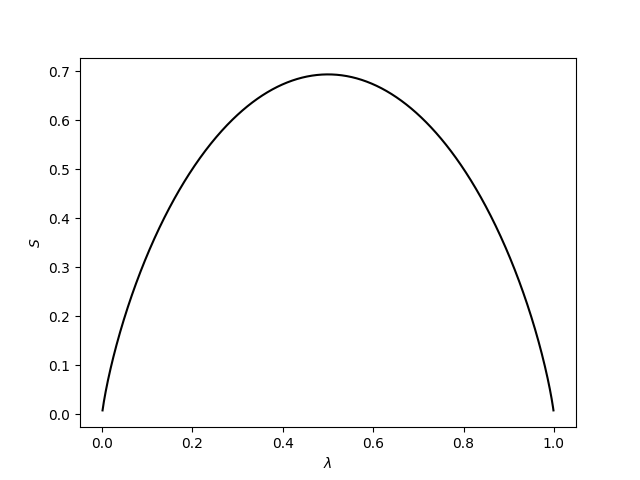
\includegraphics[width=0.7\textwidth]{entropia_M2.png}
\caption{The entropy of equation \ref{eq:entropy_M2} as a function of the probability that the photon has horizontal polarization.}
\end{figure}
\end{example}

\section{Von Neumann Algebras}

In this section we will explore the theory of von Neumann algebras. Although these are special cases of $C^*$-algebras, they will be the correct setting to develop Tomita-Takesaki theory and eventually connect it with KMS states. Moreover, their study is also important for the general theory of quantum systems with infinite degrees of freedom including quantum field theories\cite{Haag1996}. In this case, to be concrete we will follow the presentation of \cite{ Evans1998}. 

\begin{definition}
Let $\mathfrak{M}\subseteq \mathcal{B}({\mathcal{H}})$ for some Hilbert space $\mathcal{H}$. The commutant of $\mathfrak{M}$ is
\begin{equation}
\mathfrak{M}'=\{A\in\mathcal{B}(\mathcal{H})|AB=BA\text{ for all } B\in\mathfrak{M}\}.
\end{equation}
We say $\mathfrak{M}$ is a von Neumann algebra ($W^*$-algebra) if $\mathfrak{M}''=\mathfrak{M}$.
\end{definition}

\begin{example}
It is clear that for all $\mathfrak{M}\subseteq\mathcal{B}(\mathcal{H})$ for some Hilbert space $\mathcal{H}$ we have $\mathfrak{M}\subseteq\mathfrak{M}''$. Therefore $\mathcal{B}(\mathcal{H})$ is a $W^*$-algebra.
\end{example}

We claimed that every $W^*$-algebra is a $C^*$-algebra. Indeed,

\begin{theorem}
Let $\mathfrak{M}\subseteq \mathcal{B}({\mathcal{H}})$ for some Hilbert space $\mathcal{H}$ be self-adjoint. Then $\mathfrak{M}'$ is a $C^*$-algebra.
\end{theorem}

\begin{proof}
It is a matter of checking that $\mathfrak{M}'$ is a *-algebra. It is clear that for all $A\in\mathfrak{M}'$ we have $\|A^*A\|=\|A\|^2$ since this is true in $\mathcal{B}(\mathcal{H})$. Finally, if $(A_n)$ is a Cauchy sequence in $\mathfrak{M}'$ then it converges to some $A\in\mathcal{B}(\mathcal{H})$. Since multiplication is continuous (a simple consequence of the compatibility between multiplication and the norm in $C^*$-algebras and therefore in $\mathcal{B}(\mathcal{H})$) we have that
\begin{align}
\begin{split}
AC&=(\lim_{n\rightarrow\infty}A_n)C = \lim_{n\rightarrow\infty}A_nC=\lim_{n\rightarrow\infty}CA_n \\
&= C\lim_{n\rightarrow\infty}A_n=CA.
\end{split}
\end{align}
Therefore $\mathfrak{M}'$ is Banach and we conclude it is a $C^*$-algebra.
\end{proof}

\begin{corollary}\label{cor:W_C}
A $W^*$-algebra is a $C^*$-algebra.
\end{corollary}

\begin{theorem}
Let $\mathfrak{M}$ be a von Neumann algebra on a Hilbert space $\mathcal{H}$ and $G\subseteq\mathcal{H}$. Then $G$ is cyclic for $\mathfrak{M}$ if and only if $G$ is separating for $\mathfrak{M}'$.
\end{theorem}

\begin{proof}
Suppose $G$ is cyclic for $\mathfrak{M}$ and let $A\in\mathcal{M}'$ be such that $AG=\{0\}$. Then for all $\mathcal{B}\in\mathfrak{M}$ and $x\in G$ we have $ABx=BAx=B0=0$. By continuity $A=0$.
Conversely, suppose $G$ is separating for $\mathfrak{M}'$ and let $P$ be the orthogonal projection on $\overline{\mathfrak{M}G}$. We will prove that the projection onto its orthogonal complement is null. First note that $P\in\mathfrak{M}'$. Indeed, if $x\in\mathcal{H}$ there exists $y\in \overline{\mathfrak{M}G}$ and $z\in\overline{\mathfrak{m}G}^\bot$ such that $x=y+z$. If $A\in\mathfrak{M}$ then $Ay\in\overline{\mathfrak{M}G}$ and $APy=Ay=PAy$. On the other hand, $Az\in\overline{\mathfrak{m}G}^\bot$ since for all $v\in\overline{\mathfrak{m}G}$ we have $\langle v,Az\rangle=\langle A^*v,z\rangle=0$. Therefore $PAz=0=A0=APz$. We conclude that $PAx=APx$ and $P\in\mathfrak{M}'$.Then it is clear that $1-P\in\mathfrak{M}'$ and we have $(1-P)G=\{0\}$. Since $G$ is separating for $\mathfrak{M}'$ we have $1-P=0$ and therefore $P=1$ showing that $G$ is cyclic for $\mathfrak{M}$.
\end{proof}

As it turns out, the GNS representation of a von Neumann algebra equipped with a faithful normal state will have properties which as we will see later are suitable for the application of Tomita-Takesaki theory.

\begin{theorem}\label{thm:GNS_von}
Let $\mathfrak{M}$ be a $W^*$-algebra and $\omega$ be a normal faithful state. Then the GNS representation $(\mathcal{H}_\omega,\pi_\omega)$ is faithful, $\pi_\omega(\mathfrak{M})$ is a $W^*$-algebra and the cyclic vector $\Omega_\omega$ is separating for $\pi_\omega(\mathfrak{M})$.
\end{theorem} 

\begin{proof}
The fact that $\pi_\omega(\mathfrak{M})$ is a $W^*$-algebra is given in \cite{Bratteli1997} and relies on the topological properties of von Neumann algebras which we have not discussed. Let $A\in\mathfrak{M}$ be such that $\pi_\omega(A)\Omega_\omega=0$ (which in particular is true if $A\in\ker\pi_\omega$). Then since $\omega$ is faithful and
\begin{equation}
\omega(A^*A)=\langle \Omega_\omega, \pi_\omega (A^*A)\Omega_\omega\rangle=\langle \pi_\omega(A)\Omega_\omega,\pi_\omega(A)\Omega_\omega\rangle=0
\end{equation}
we conclude that $A^*A=0$. Therefore by the $C^*$-property $0=\|A^*A\|=\|A\|^2$ and $A=0$. We conclude that the representation is faithful and $\Omega_\omega$ is separating for $\pi_\omega(\mathfrak{M})$.
\end{proof}

\section{Dynamical Systems}

Up until now, we have only focused on the description of observables and states of a physical system. In no way have we yet discussed the dynamics of a system. In the context of algebraic physics we have that the concept of time evolution is implemented through automorphisms of the algebra of observables. To show this we will follow \cite{Duvenhage1999}.

\begin{definition}\label{def:dynamics}
Let $\mathcal{A}$ be a $C^*$-algebra. A one-parameter automorphism group is a group homomorphism $\tau:\mathbb{R}\rightarrow \Aut(\mathcal{A})$ $t\mapsto\tau_t$. If $\tau$ is a one-parameter automorphism group where the map $\mathbb{R}\rightarrow\mathcal{A}$ given by $t\mapsto\tau_t(A)$ is continuous for all $A\in\mathcal{A}$, then $(\mathcal{A},\tau)$ is called a $C^*$-dynamical system. If $\mathfrak{M}$ is a $W^*$-algebra on a Hilbert space $\mathcal{H}$ and $\tau$ is a one-parameter automorphism group on $\mathfrak{M}$ such that $\mathbb{R}\rightarrow\mathcal{H}$ given by $t\mapsto\tau_t(A)x$ is continuous for all $A\in\mathfrak{M}$ and $x\in\mathcal{H}$, then $(\mathfrak{M},\tau)$ is called a $W^*$-dynamical system. 
\end{definition}

The distinction we make for von Neumann algebras reflects the fact that even though we have corollary \ref{cor:W_C}, von Neumann algebras will be more general in physical applications. Indeed we have,

\begin{theorem}\label{thm:C_W}
A $C^*$-dynamical system whose underlying algebra is a $W^*$-algebra is a $W^*$-dynamical system.
\end{theorem}

\begin{proof}
Let $\mathfrak{M}$ be a $W^*$-algebra on a Hilbert space $\mathcal{H}$ and $(\mathfrak{M},\tau)$ a $C^*$-dynamical system. Notice that for every $x\in\mathcal{H}$ the evaluation map $\ev_{x}:\mathfrak{M}\rightarrow \mathcal{H}$ given by $\ev_{x}(A)=Ax$ is continuous. Indeed if $\epsilon\in\mathbb{R}^+$, $\delta=\epsilon/\|x\|$, and $\|A-B\|<\delta$ for $A,B\in\mathfrak{M}$ then
\begin{equation}
\|Ax-Bx\|=\|(A-B)x\|\leq\|A-B\|\|x\|<\frac{\epsilon}{\|x\|}\|x\|=\epsilon.
\end{equation}
Then the map $\mathbb{R}\rightarrow\mathcal{H}$ $t\mapsto\tau_t(A)x$, being $\ev_{x}$ after $\mathbb{R}\rightarrow\mathcal{A}$ $t\mapsto\tau_t(A)$ continuous by hypotheses, is continuous for all $A\in\mathfrak{M}$ and $x\in\mathcal{H}$. The conclusion follows.
\end{proof}

Following \cite{Duvenhage1999} we will from now on restrict to finite dimensional Hilbert spaces to inspire notions which we will however generalize later by using definition \ref{def:dynamics}.

\begin{example}\label{ex:schrodinger}
In quantum mechanics we already have a dynamical law given by Schrödinger's equation. Consider a finite dimensional Hilbert space $\mathcal{H}$ with a self-adjoint Hamiltonian $H$. The time evolution, as prescribed by Heisenberg's representation of Schrodinger's mechanics is the restriction of
\begin{alignat}{2}
\tau:\mathbb{C}&\rightarrow&\Aut(\mathcal{B}(\mathcal{H})) \nonumber \\
z&\mapsto&\tau_z:\mathcal{B}(\mathcal{H})&\rightarrow\mathcal{B}(\mathcal{H}) \\
&&A&\mapsto e^{iHz}Ae^{-iHz} \nonumber
\end{alignat}
to the real numbers. The verification that this map is well defined and indeed restricts to a one-parameter automorphism group is routine.
Let $\{e_1,\dots,e_N\}$ be an orthonormal basis of eigenvectors of $H$ associated to the eigenvalues $E_1,\dots,E_N$ (whose existence is guaranteed by the spectral theorem). Then we have
\begin{align}
\begin{split}
\|e^{iHt}-1\|&=\|\sum_{n=1}^Ne^{iE_nt}\rho_{e_n}-\sum_{n=1}^N \rho_{e_n}\|\leq\sum_{n=1}^N \|\left(e^{iE_nt}-1\right)\rho_{e_n}\| \\
&= \sum_{n=1}^N|e^{iE_nt}-1|\|\rho_{e_n}\|=\sum_{n=1}^N|e^{iE_nt}-1|\rightarrow 0
\end{split}
\end{align}
as $t\rightarrow 0$. Therefore if $s\in\mathbb{R}$ we have
\begin{align}
\begin{split}
\lim_{t\rightarrow s}\tau_t(A)=\lim_{t\rightarrow s}\tau_{t-s}\tau_s(A)=\lim_{t\rightarrow s}e^{iH(t-s)}\tau_s(A)e^{iH(s-t)}=\tau_s(A)
\end{split}
\end{align}
for all $A\in \mathcal{B}(\mathcal{H})$. We conclude that $(\mathcal{B}(\mathcal{H}),\tau)$ is a $C^*$ and $W^*$-dynamical system.
\end{example} 

Note that even though the dynamics have been defined through automorphisms of the algebra resembling Heisenberg's quantum mechanics, we could have equally defined it analogously to Schrodinger's mechanics through the evolution of states
\begin{equation}
\tau_t(\omega)(A):=\omega(\tau_t(A)).
\end{equation}
This yields the same physics and we will occasionally use it to give a physical interpretation to mathematical results. 

The following consequence given in \cite{Duvenhage1999} of having a state invariant under the dynamics of a system for its GNS representation will be useful later on to formulate the connection between KMS states and Tomita-Takesaki theory.

\begin{theorem}
Let $\mathcal{A}$ be a $C^*$-algebra, $\tau$ a one-parameter group of automorphisms of $\mathcal{A}$, $\omega$ a state such that $\omega(\tau_t(A))=\omega(A)$ for all $t\in\mathbb{R}$ and $A\in\mathcal{A}$, and $(\mathcal{H}_\omega,\pi_\omega)$ the induced GNS representation. Then there exists a unique one-parameter unitary group
\begin{align}
\begin{split}
U:\mathbb{R}&\rightarrow\{A\in\mathcal{B}(\mathcal{H})|A\text{ is unitary}\} \\
t&\mapsto U_t
\end{split}
\end{align}
such that $U_t\Omega_\omega=\Omega_\omega$ and $\pi_\omega(\tau_t(A))=U_t\pi_\omega(A)U_{-t}$ for all $t\in\mathbb{R}$ and $A\in\mathcal{A}$. Furthermore, if $(\mathcal{A},\tau)$ is a $W^*$-dynamical system and $\pi_\omega(\mathcal{A}$ is a von Neumann algebra, then $U$ is strongly continuous.
\end{theorem} 